%! Author = noOne
%! Date = 3/9/22

% Preamble
\documentclass[11pt]{article}

% Packages
\usepackage{amsmath}
\usepackage{blindtext}
\usepackage{graphicx}
\usepackage{csquotes}

%
\title{Neuroanatomy and Perceptrons}
\author{noOne}
\date{\today}

% Document
\begin{document}
\maketitle{Neuroanatomy and Perceptrons}
\section{Week 1: Overview}\label{sec:week-1:-overview}
In this first lesson, we will look at the historical background of artificial intelligence and deep learning, biological and artificial neurons, the perceptron learning algorithm, and the training of multi-layer neural networks by gradient descent.
We will briefly review certain topics from probability which are essential for deep learning, and we will introduce the issue of generalization and overfitting in supervised learning.

\section{Weekly learning outcomes:}\label{sec:weekly-learning-outcomes:}
By the end of this week, you will be able to:

\begin{itemize}
    \item construct perceptrons by hand
    \item apply the Perceptron Learning Algorithm
    \item construct multi-layer perceptrons by hand
    \item explain how continuous activation functions allow multi-layer neural networks
to be trained by gradient descent
    \item compute Entropy and KL-Divergence for discrete probability distributions
    \item compute probabilities using Bayes’ Rule.
    \item describe the basics of supervised learning.
    \item explain how to avoid overfitting in neural networks.
\end{itemize}

\pagebreak

\section{History Neuroanatomy}\label{sec:history--neuroanatomy}

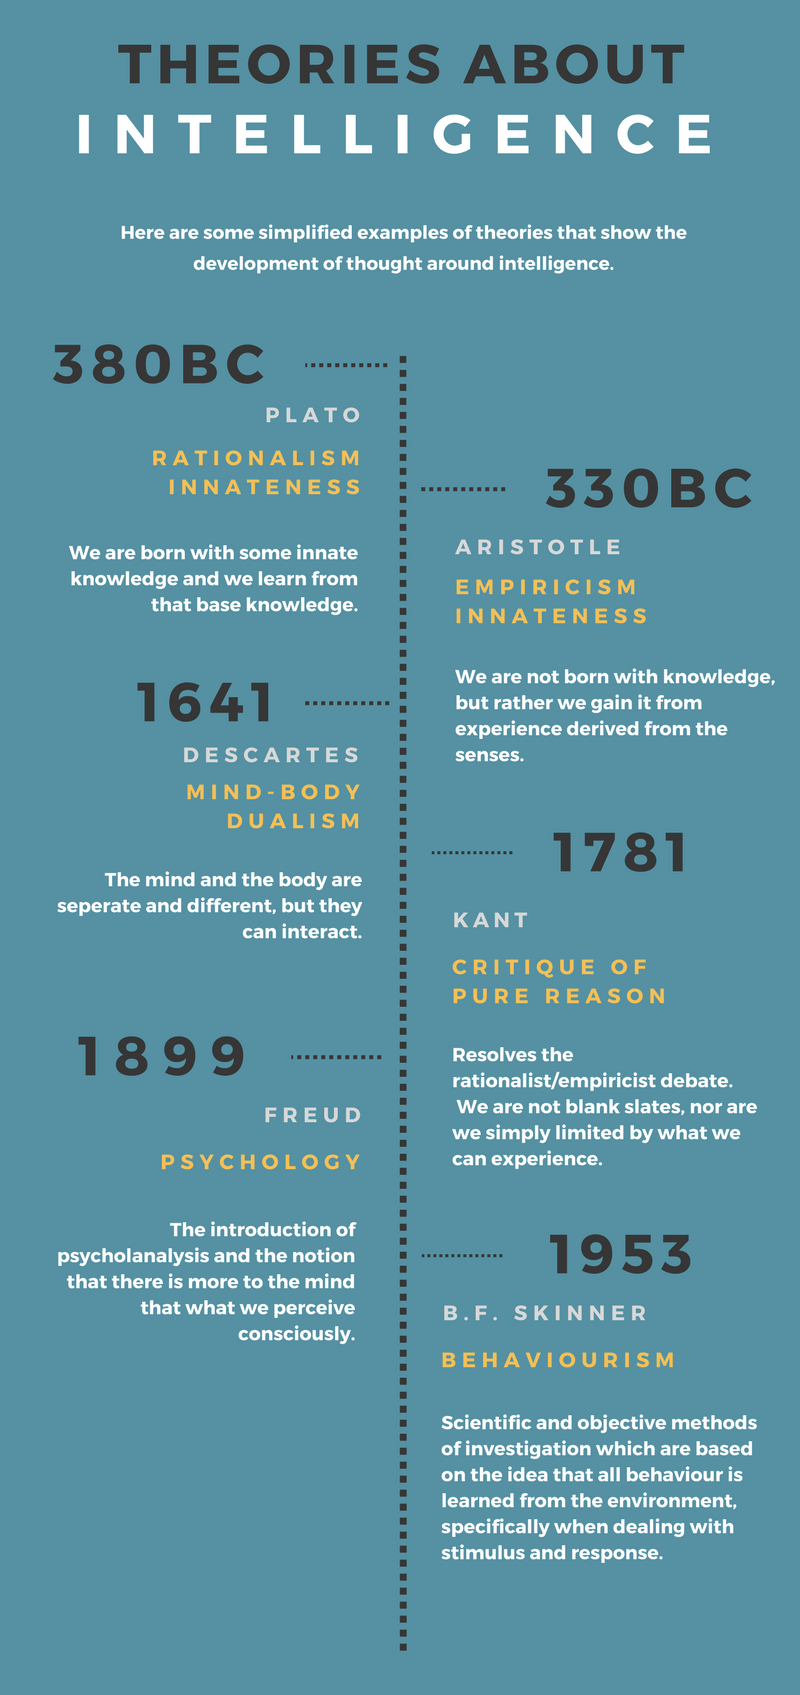
\includegraphics[width=\textwidth,height=\textheight,keepaspectratio]{images/img}

\begin{displayquote}
\emph{``For the machine is not a thinking being, but simply an automation which acts
according to the laws imposed upon it.'}
\textbf{Ada Lovelace, 1843}
\end{displayquote}

The table above summarizes various theories which have been proposed throughout history to explain the workings of the human mind.
The idea that human reasoning could be simulated by some kind of mechanical calculator dates back to Blaise Pascal and Gottfried Leibniz in the 1600's, was developed in the 1800's by George Boole, Gottlob Frege, Charles Babbage and Ada Lovelace, and in the early 1900's by Alan Turing.

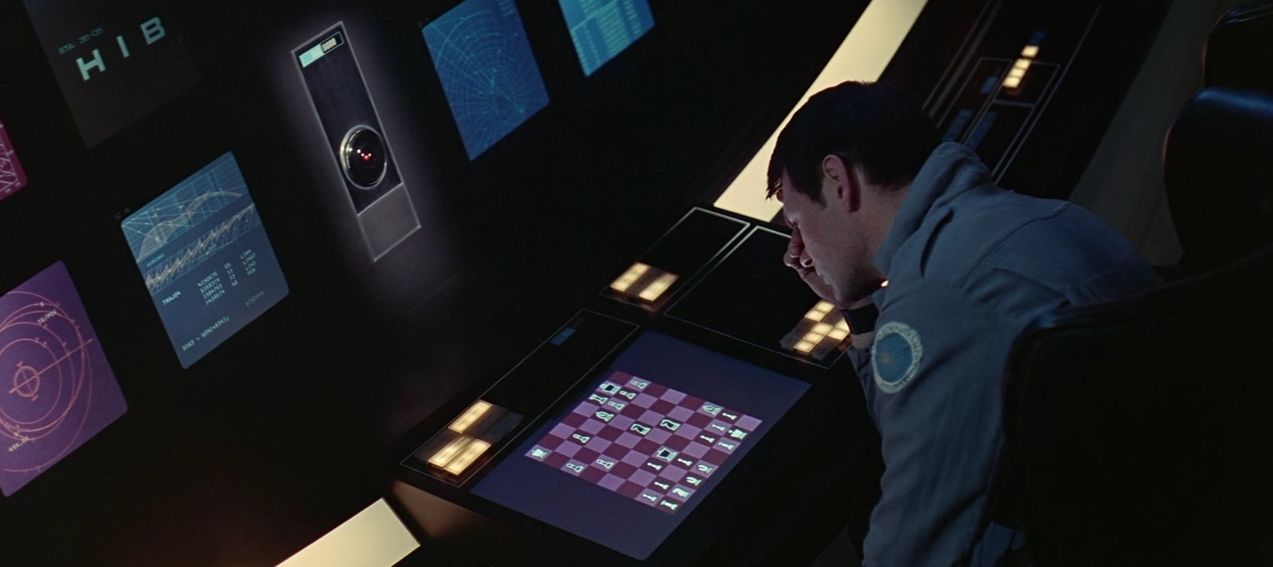
\includegraphics[width=\textwidth]{images/img_1}
The modern field of Artificial Intelligence (AI) perhaps began in earnest with a workshop at Dartmouth College in the summer of 1956.
In the early days of AI, researchers tended to focus on logical reasoning and problem-solving.
Less attention was paid to perceptual tasks such as vision and language processing, because there was a general expectation that these tasks would be easily solved within a few years.
In reality, these seemingly simple tasks turned out to be much more challenging, and were not achieved to any degree of proficiency until the second decade of the 21st Century.
The major advances in these areas stem chiefly from a class of models called Deep Neural Networks which are inspired by the structure of the human brain.

\section{sub symbolic processing}\label{sec:sub-symbolic-processing}
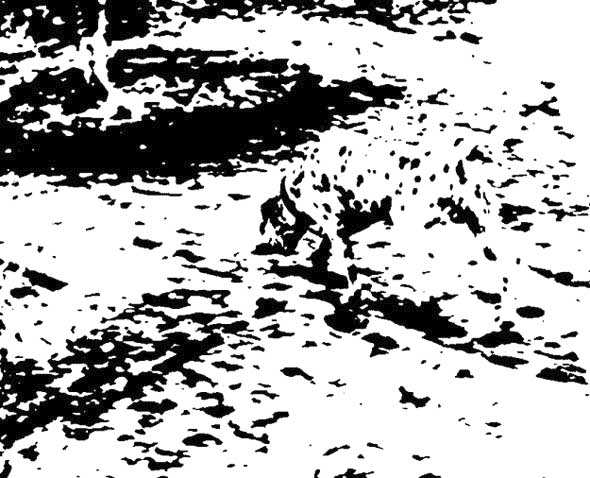
\includegraphics[width=\textwidth,height=\textheight,keepaspectratio]{images/img_2}
Can you see an animal in this picture?
What kind of animal is it?
What direction is it facing?
The human brain performs tasks such as object recognition unconsciously and in
a highly distributed fashion.
Low-level features are recognised in different parts of the image and are hierarchically combined into high level features
from which the identity of the object is extracted.

\section{Basic Neuroanatomy}\label{sec:basic-neuroanatomy}
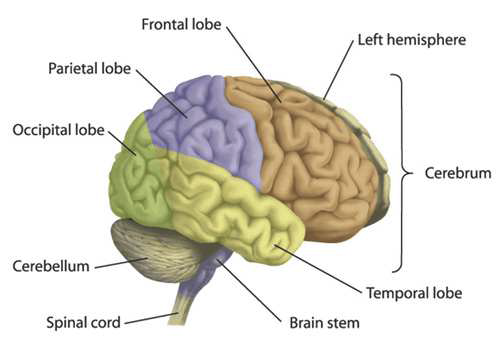
\includegraphics[width=\textwidth,height=\textheight,keepaspectratio]{images/img_3}

\section{Cerebral Cortex}\label{sec:cerebral-cortex}
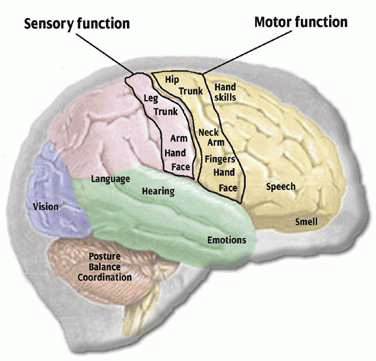
\includegraphics[width=\textwidth,height=\textheight,keepaspectratio]{images/img_4}

\section{Brain Functions}\label{sec:brain-functions}
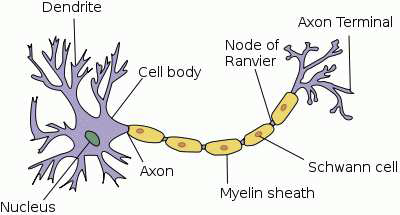
\includegraphics[width=\textwidth,height=\textheight,keepaspectratio]{images/img_5}

\section{Neurons}\label{sec:neurons}
The body is made up of billions of cells.
Cells of the nervous system, called neurons, are specialized to carry “messages” through an electrochemical process.
The human brain has about 100 billion neurons, and a similar number of support cells called “glia”.
Neurons share many functions in common with other cells in the body.
For example, they are surrounded by a cell membrane, they have a nucleus containing genes (DNA), and they  carry out basic cellular
processes like protein synthesis and energy production.

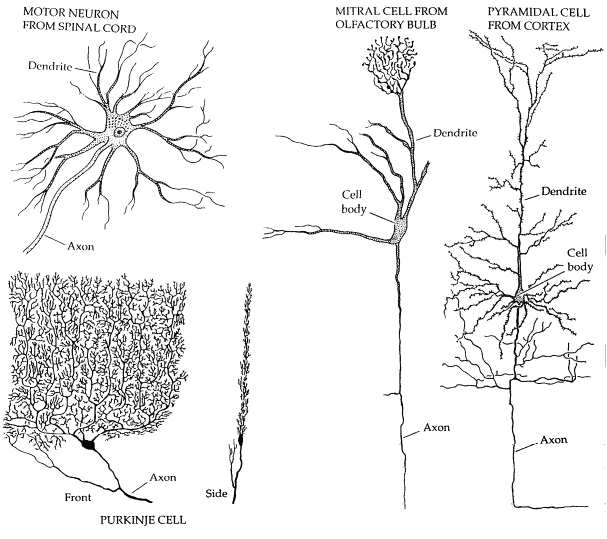
\includegraphics[width=\textwidth,height=\textheight,keepaspectratio]{images/img_6}

Neurons also have certain features which distinguish them from other body cells.
They have specialized extensions called dendrites and axons.
Dendrites bring information to the cell body, while axons take information away from the cell body.
The axon of one neuron can connect to the dendrite of another neuron through an electrochemical junction called a synapse.

\section{Variety of Neuron Types}\label{sec:variety-of-neuron-types}
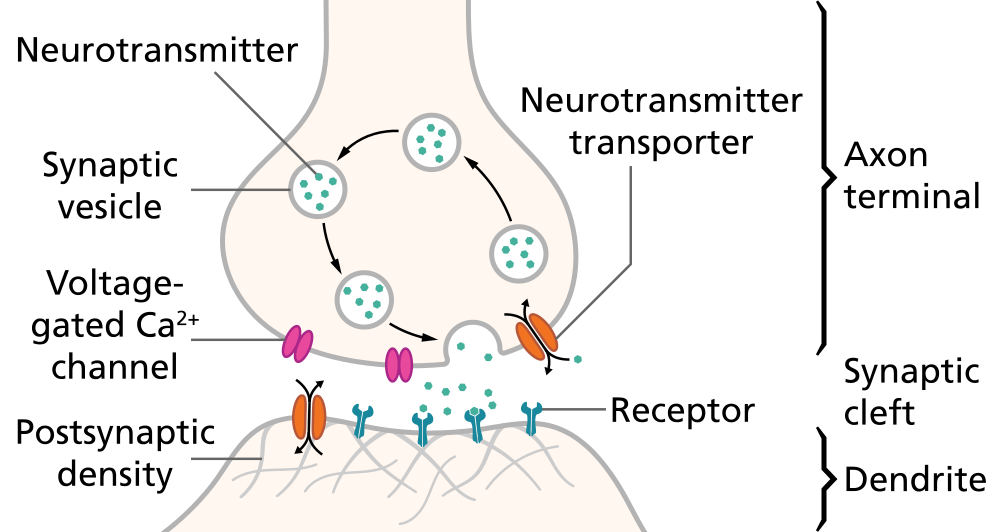
\includegraphics[width=\textwidth,height=\textheight,keepaspectratio]{images/img_7}

Most neurons have only one axon, but the number of dendrites can vary widely.
Unipolar and Bipolar neurons have only one dendrite, but Purkinje neurons in the cerebellum can have up to 100,000 dendrites.
Dendrites are typically less than a millimetre in length.
Axons can vary in length from less than a millimetre to more than a metre (for motor neurons).
Long axons are sometimes surrounded by a myelinated sheath, which prevents the electrical signal from dispersing, and allows it to travel faster (up to 100 m/s).

\section{Synapses, Neurotransmitters and Ion Channels}\label{sec:synapses-neurotransmitters-and-ion-channels}
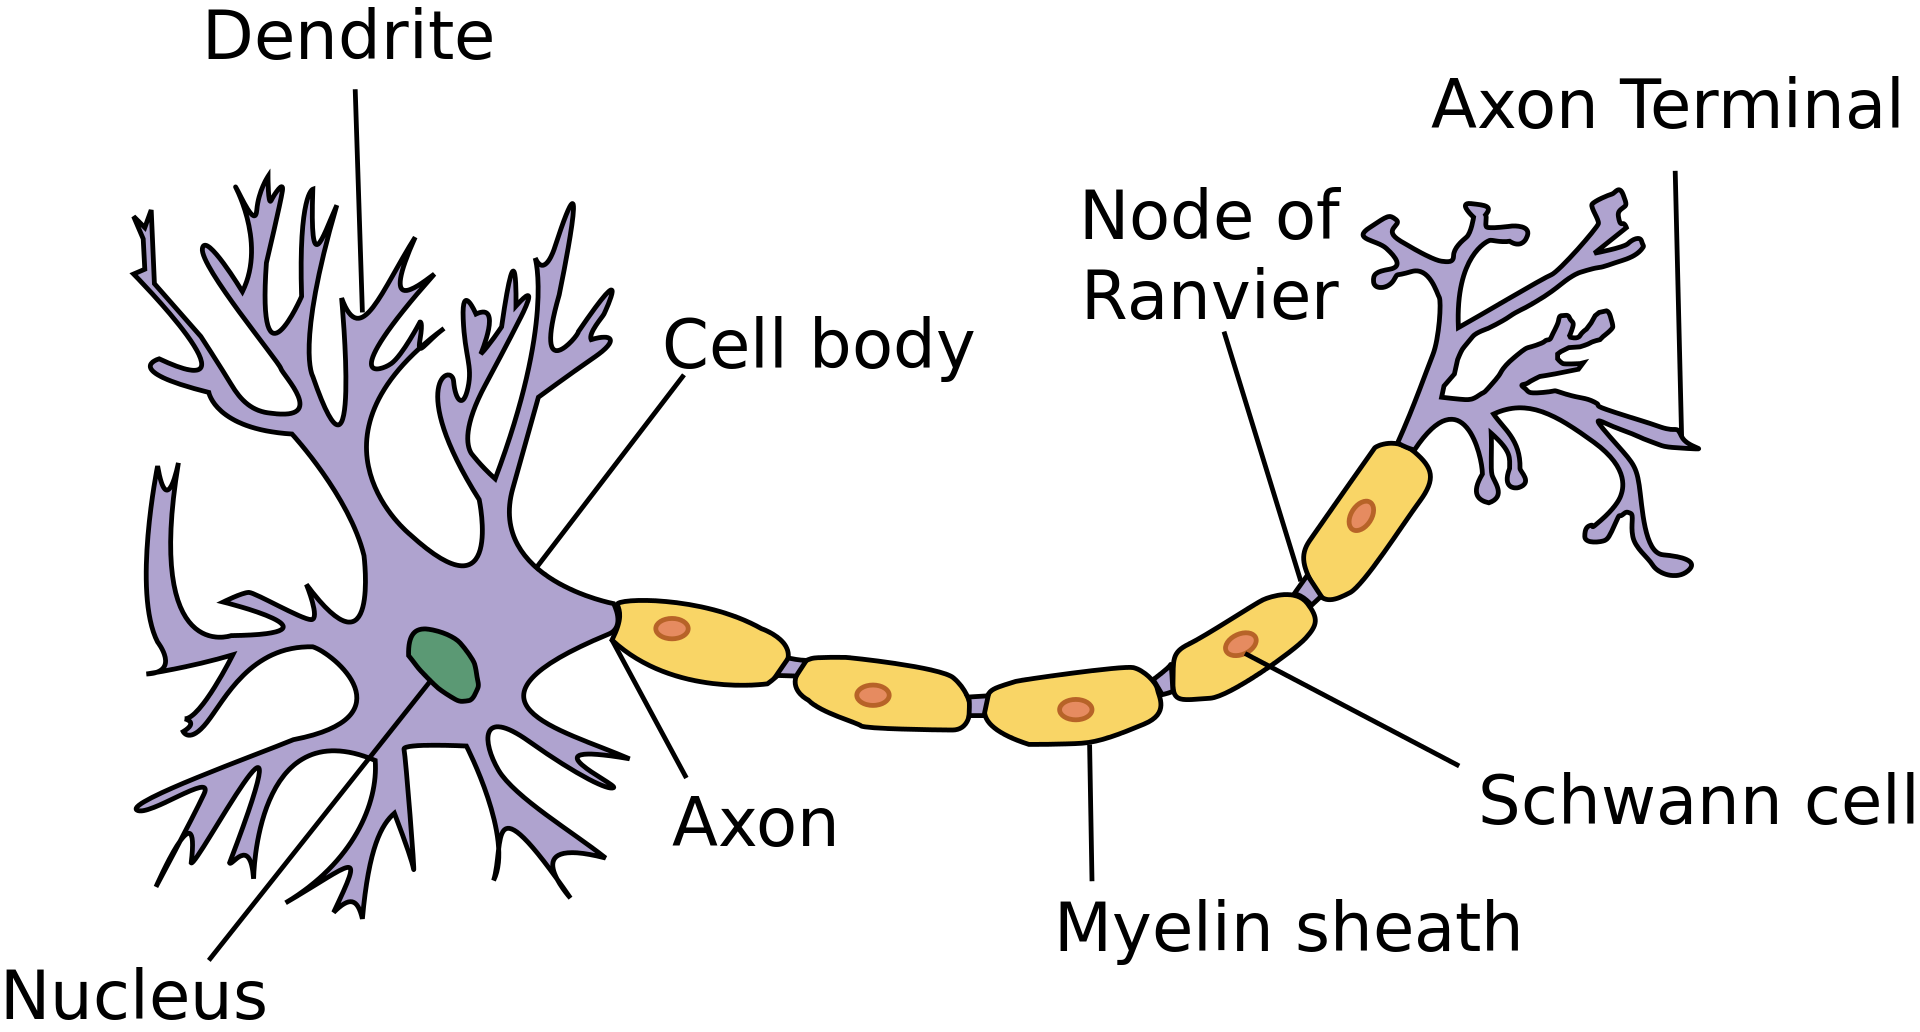
\includegraphics[width=\textwidth,height=\textheight,keepaspectratio]{images/img_8}

An electrical pulse reaches the endbulb and causes the release of neurotransmitter molecules from little packets (vesicles) through the synaptic membrane.
The transmitter passes through voltage-gated ion channels and diffuses through the synaptic cleft to the other side.

When the neurotransmitter reaches the post-synaptic membrane, it binds to receptors and causes a change in polarisation of the membrane.
The change in potential can be excitatiory (moving the potential towards the threshold) or inhibitory (moving it away from the threshold).

In the next section, we will look at a simple mathematical model of the neuron which excludes most of the complex biological, chemical and physiological details and aims instead to capture the essential features of a neuron necessary for distributed computation.

\pagebreak

\section{Further Reading}\label{sec:further-reading}
For more on the history of Deep Learning, consider these two perspectives:

\begin{itemize}
    \item Viewpoint 1: Focusing on recent work (after 2012)
    \item https://www.cs.toronto.edu/~hinton/absps/NatureDeepReview.pdf
    \item Viewpoint 2: Focusing on earlier work (before 2012)
    \item http://people.idsia.ch/~juergen/deep-learning-overview.html
    \item Textbook: Deep Learning (Goodfellow, Bengio, Courville, 2016):
    \item historical trends in deep learning
    \item https://www.deeplearningbook.org/contents/intro.html
\end{itemize}

\pagebreak

\section{Exercises: Perceptrons}\label{sec:exercises:-perceptrons}

\textbf{Question 1:}
Construct by hand a Perceptron which correctly classifies the following data.
use your knowledge of plane geometry to choose appropriate values for the weights \(w_0, w_1\) and \(w_2\).

\begin{center}
\begin{tabular}{ |c|c|c|c| }
    \hline
    \textbf{Training Example} & \textbf{\(x_1\)} & \textbf{\(x_2\)} & \textbf{Class} \\
    \hline
    a. & 0 & 1 & -1 \\
    b. & 2 & 0 & -1 \\
    c. & 1 & 1 & +1 \\
    \hline
\end{tabular}
\end{center}

Identify the equation of the line and the weights of the Perceptron (including bias).

\textbf{Explanation}
The first step is to plot the data on a 2-D graph, and draw a line which separates the positive from the negative data points:

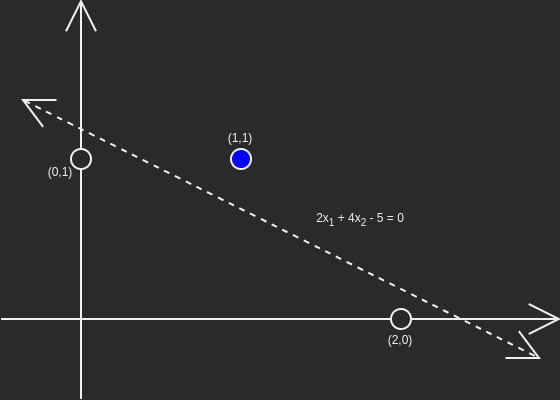
\includegraphics[width=\textwidth,height=\textheight,keepaspectratio]{images/graph_1}

This line has slope \(-\dfrac{1}{2}\) and \(x_2\)-intersect \(\dfrac{5}{4}\), so the equation is:
\(x_2 = \dfrac{5}{4} - \dfrac{x_1}{2}\)

ie \(2x_1 + 4x_2 - 5 = 0\)

Taking account of which side is positive, this corresponds to these weights:

\begin{center}
\begin{tabular}{ |c|c|c| }
    \(w_0\) & = & \(\-5\) \\
    \(w_1\) & = & \(2\) \\
    \(w_2\) & = & \(4\)
\end{tabular}
\end{center}

Alternatively, we can derive weights \(w_1 = 1\) and \(w_2=2\) by drawing a vector normal to the separating line, in the direction pointing towards the positive data points:

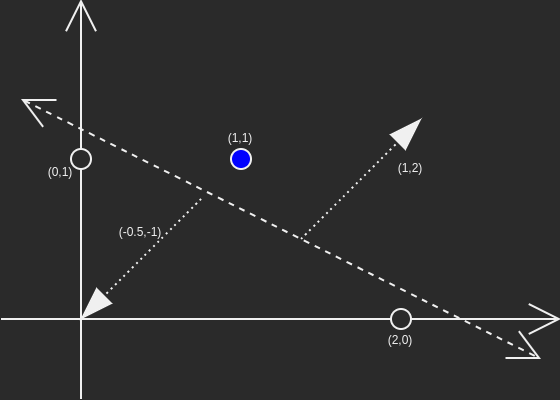
\includegraphics[width=\textwidth,height=\textheight,keepaspectratio]{images/graph_2}

The bias weight \(w_1=1\) can then be found by computing the dot product of the normal vector with a perpendicular vector from the separating line to the origin.
In this case \(w_0 = 1(-0.5) + 2(-1) = -2.5\)

(Note: these weights differ from the previous ones by a normalising constant, which is fine for a perceptron)

\pagebreak

\textbf{Question 2:}Demonstrate the Perceptron Learning Algorithm on the above data, using a learning rate of 1.0 and initial weight values of
\begin{center}
\begin{tabular}{ c c c }
    \(w_0\) & = & -1.5 \\
    \(w_1\) & = & 0 \\
    \(w_2\) & = & 2
\end{tabular}
\end{center}

The first three steps are shown below.
You should continue until all items are correctly classified.

\begin{center}
\begin{tabular}{ |c|c|c|c|c|c|c|c|c|c| }
    \hline
    Iteration & \(w_0\) & \(w_1\) & \(w_2\) & Item & \(x_1\) & \(x_2\) & Class & \(s = w_0 + w_1 x_1 + w_2 x_2\) & Action \\
    \hline
    1 & -1.5 & 0 & 2 & a & 0 & 1 & -1 & +0.5 & subtract \\
    2 & -2.5 & 0 & 1 & b & 2 & 0 & -1 & -2.5 & None \\
    3 & -2.5 & 0 & 1 & c & 1 & 1 & +1 & -1.5 & Add \\
    \hline
\end{tabular}
\end{center}

\textbf{Explanation}
\begin{center}
\begin{tabular}{ |c|c|c|c|c|c|c|c|c|c| }
    \hline
    Iteration & \(w_0\) & \(w_1\) & \(w_2\) & Item & \(x_1\) & \(x_2\) & Class & \(s = w_0 + w_1 x_1 + w_2 x_2\) & Action \\
    \hline
    1 &
    2 &
    3 &
    4 &
    5 &
    6 &
    7 &
    8 &
    9 &
    10 &
    11 &
    12 &
    \hline
\end{tabular}
\end{center}

\end{document}